% Template for ISBI-2018 paper; to be used with:
%          spconf.sty  - ICASSP/ICIP LaTeX style file, and
%          IEEEbib.bst - IEEE bibliography style file.
% --------------------------------------------------------------------------
\documentclass{article}
\usepackage{spconf,amsmath,graphicx}
\usepackage{caption}

\usepackage[utf8]{inputenc}
\setcounter{page}{1}
\thispagestyle{plain}
\pagestyle{plain}

% Example definitions.
% --------------------
\def\x{{\mathbf x}}
\def\L{{\cal L}}

% Title.
% ------
\title{Advanced Image Analysis Project: A Python Package (IMMAS) for Mass Detection in Digital Mammograms}
%
% Single address.
\name{Brianna Burton, Doiriel Vanegas, Mahlet Birhanu, Marcio A. B. C. Rockenbach, Oleh Kozynets}
\address{\textit{Supervior: Professor Alessandro Bria}\\
    MAIA Master: University of Cassino and Southern Lazio\\
	Via Di Biasio, 43\\
	03043 Cassino (FR)}% ---------------


\begin{document}
%\ninept
%
\maketitle
%
\begin{abstract}
Breast cancer ranks among the most deadly diseases worldwide and is a constant threat to women's health. Imperative to survival is early and accurate diagnosis through screening. As the medical world evolves into the digital era, radiologists can be aided by a second opinion using computer aided diagnosis (CAD) systems. As such, this report presents an Intelligent Mammogram Mass Analysis and Segmentation (IMMAS) module for mass detection. It explains the optimal advanced image processing and pattern recognition techniques required for segmentation and classification of masses in breast mammogram images. Experiments are performed on the dataset INbreast, a publicly available dataset. Images are first preprocessed using intensity based transforms and then segmented using multithresholding. The resulting binary image is used to extract geometric and intensity-based features from regions, as well their local binary patterns (LBP). Two classifiers, support vector machine (SVM) and random forest (RF), are used to detect the masses and are compared using a free-response receiver operating characteristic curve (FROC) with a optimal area under the curve (AUC) from 0 to 1 of 0.59. This investigation results in the IMMAS module, which lays the basis for a competitive CAD system.
\end{abstract}

%
\pagenumbering{arabic}
\section{Introduction}
\label{sec:intro}
\subsection{Breast Cancer}
Breast cancer is the most commonly diagnosed cancer among women, with approximately 182,000 women diagnosed with the condition annually in the United States \cite{Jemal2009}. Every year, around 40,000 women die of breast cancer, making it the second-leading cause of cancer death among American women after lung cancer.\par
Clinical symptoms of breast cancer include change in breast size or shape, skin changes, nipple abnormalities, single-duct discharge, and axillary lumps \cite{Chalasani2018}. However, those symptoms usually appear late in the course of disease, reflecting advanced staging and less chance of cure. To be able to detect cancer in earlier stages, mammograms must be used.\par

\subsection{Mammograms}
Mammography is a radiographic technique for imaging of the breast. It is used for screening and diagnostic purposes. In both cases, the technique is similar. Four images are acquired, two for each breast, one being medio-lateral oblique view and another craniocaudal view. If necessary, more specific views can be obtained, according to the orientation given by the radiologist. Mammograms have an overall sensibility around 88-93\% and specificity between 85-94\% \cite{Saude2007}. Therefore, they form an excellent method for early diagnosis of breast cancer. \par
An exam report is based on the BI-RADS system \cite{Sickles2013}. BI-RADS was designed to standardize breast imaging reporting and to reduce confusion in breast imaging interpretations. It is also an important tool that allows outcome monitoring and quality assessment. The classification by the BI-RADS varies between categories from 0 to 6. Category 0 indicates the necessity for further imaging investigation, and 6 indicates a mammogram already known to be positive for cancer. The categories between 1 and 5 indicate the risk for cancer, category 1 being very low and 5 very high.\par
The definition of the category relies on the imaging findings. The most common features evaluated by the radiologist include masses, calcifications, architectural distortions, asymmetries, lymphadenopathy. Those findings might be very easy or very hard to be detected, according to their characteristics and the breast composition. Therefore, it is of great clinical value to develop systems that can automatically detect suspicious areas, drawing the radiologist's attention to possible abnormalities. In the presented project, a computer aided diagnosis (CAD) system was developed to detect masses in mammograms.\par
\section{Materials}
\label{sec:materials}
\subsection{Database}
This project uses a mammographic research database called INbreast \cite{Moreira2012}. The use of a publicly known database adds legitimacy to our system, since the results can easily be compared to current and future work with this INbreast.\par
The database was acquired between 2008 and 2010, using MammNovation Siemens FFDM. It consists on images from screening, diagnostic, and follow-up exams. In total, the database has 410 images. It also contains samples with various breast densities, one of the main characteristics that affects abnormality detection (breasts with high density are harder to evaluate). In 56 cases, a biopsy was performed, of which 11 were benign and 45 were malignant.\par
The dataset contains examples of normal mammograms, mammograms with masses, mammograms with calcifications, architectural distortions, asymmetries and images with multiple findings. A mass, the subject of this project, is defined by the BI-RADS as a three-dimensional structure demonstrating convex outward borders, usually evident on two orthogonal views \cite{Sickles2013}.\par
The most significant characteristic of this database is the groundtruth annotation. While most of the databases only give a circle around the region of interest (ROI), INbreast provides the exact contour of each mass, made by a specialist in the field and validated by a second specialist. There are 115 masses among 107 images ($\sim$1.1 masses per image). The average mass area is 479 mm$^2$ (standard deviation: 619 mm$^2$, range: 15 mm$^2$ to 3689 mm$^2$). The careful and precise annotation of the contours of the masses is a great tool to simplify performance evaluation. \par
The dataset contains 16-bit images in \texttt{.tif} format, with matrix size ranging from 2560 x 3328 to 3328 x 4084 pixels. For every image, there are two binary masks: one with the entire breast tissue (to remove the background) and another with the pectoral muscle. For the images with masses, there is also a binary groundtruth image.\par

\section{Methods}
\label{sec:method}
The proposed system operates in four stages: (1) preprocessing based on morphological enhancement and wavelet transform, (2) mass candidate generation through segmentation, (3) feature extraction, and (4) false positive reduction using support vector machines (SVM) and random forest (RF) classifiers. 
\subsection{Preprocessing}
Since masses are embedded in the mammary tissue, preprocessing is necessary to separate them from the surroundings. Different preprocessing methods have been considered in the literature to enhance mass like patterns such as Morphological Enhancement, Wavelet Transforms, and Contrast Limited Adaptive Histogram Equalization (CLAHE). For this work, a combination of these techniques was applied. In a first step, bright areas are added to the image (top hat transform) while subtracting the dark areas (bottom hat transform). As a result, there is an enhancement in the contrast between bright and dark areas. To improve the contrast even more, CLAHE is applied. At the end of the preprocessing step, we perform single level 2D wavelet transform followed by median filtering and reconstruction by inverse wavelet transform.

\subsection{Segmentation}
Once the image has been enhanced, multithresholding is applied to distinguish between breast tissue, potential masses, and the background, and the image is thresholded using the largest threshold. Through this, mass candidates are found. To improve the segmentation, morphological operations are performed. The morphological parameters are chosen to maximize the Jaccard Index calculated for a segmented mammogram and the corresponding groundtruth image. In later steps, the mass candidate will be classified as positive or negative.

\subsection{Feature Extraction}
In the third step, mass candidates are described using six different groups of features as stated in Table \ref{tab:features}. A more detailed explanation of the shape, margin, texture and statistical descriptors is provided by Dong \cite{Dong2015}.

The use of Local Binary Patterns (LBP) has been reported as a good method for feature extraction in facial detection. Oliver et al. \cite{Oliver2007} proposed a method for applying LBP for false positive reduction in mass detection, by testing the performance of the LBP descriptor with different parameters for the number of neighbors $P$, the radius $R$ and for different window sizes to divide each ROI (grid size). Berbar et al. \cite{Berbar2012} performed experiments on the effect of varying the grid size in the accuracy of the classifier. Based on their best results an operator was designed with $P=8$, $R=1$, $LBP^{_{8,1}^{riu2}}$ and a $5\times5$ grid size. For each grid, 10 features are obtained, and the total number of features depends on the ROI size. Berbar suggests to use a ROI size of $256\times256$, obtaining 26,010 features, a value that is too high considering the low number of images available in our dataset. It was decided to limit the number of features to 1,000. To accomplish this, a ROI size of $50\times50$ was chosen.  

\begin{table*}[ht]
\centering
\caption{List of image descriptors}
\label{tab:features}
\begin{tabular}{llll}
\\ [-1.75ex] \cline{1-2} \\ [-1.75ex]
\textbf{Category}                                          & \textbf{Features}                                                             &  &  \\ [0.75ex] \cline{1-2} \\ [-1.5ex]
\textbf{Shape: Geometric}                                  & Perimeter, area, circularity, area/circularity ratio, shapefactor, NCPS       &  &  \\
\textbf{Shape: NRL}                                        & NRL mean, NRL SD, SD NRL/mean radial length (RL) ratio, NR entropy            &  &  \\
\textbf{Margin Gradient}                                   & Gradient: mean, SD, skewness                                                  &  &  \\
\textbf{Texture: Grey Level Histogram}                     & Intensity: mean, standard deviation, smoothness, skewness, kurtosis           &  &  \\
\textbf{Statistical: Grey Level Co-occurance Matrix}       & Correlation, contrast, uniformity, homogeneity, energy, dissimilarity         &  &  \\
\textbf{Whole image}                                      & Local Binary Patterns (LBP)                                                   &  &  \\ [0.75ex] \cline{1-2} \\ [-1.75ex]
\multicolumn{2}{l}{\textit{NRL normalized radial length, NCPS normalized central position shift, RL radial length, SD standard deviation}} &  & 
\end{tabular}
\end{table*}

\subsection{Machine Learning}
In the last step, two classifiers are built: a support vector machine (SVM) and a random forest (RF), to be compared later. First, the dataset is divided randomly into two subsets (train and test) in equal proportions. The division is done so that regions belonging to the same image were assigned to the same subset (training or test). Then, a 2-fold-cross-validation strategy is used.\par
The classifier is also run under two different conditions: one using all the features and another using all features except LBP to test the effect of the dominating feature, LBP, on the resulting classifier.\par

\subsubsection{Support Vector Machine (SVM)}
Support vector machines consist of a learning model for classification and regression problems. Given a set of features and their corresponding classes, this classifier builds a hyperplane to separate features related to different classes. The best result is given by the maximum margin hyperplane, named the optimal separating hyperplane (OSH). The linear discriminant function of this OSH is called support vector machine.\par
The scikit-learn library is used to create and test an SVM classifier. The performance of the classifier is initially evaluated by the area under the ROC curve. This score is used in several grid searches to find the best possible hyperparameters, using different kernels (linear, rbf, sigmoid, polynomial), values of C (penalty to errors), classes weight and values of gamma. The hyperparameters with the best performance are used to build the final classifier.\par

\subsubsection{Random Forest (RF)}
The random forest classifier creates ensemble of independent decision trees, where every tree is built by random selection of features \cite{Breiman2001}. Each tree is a weak classifier. In the process of classification, the final decision is obtained as a result of the majority vote. This classifier is more robust with respect to noise than other ensemble classifiers.

The random forest classifier implementation is provided by the scikit-learn library. Because the classification of mammogram ROIs is a quite unbalanced problem, class weights were automatically adjusted inversely proportional to class frequencies in the input data \cite{Pedregosa2011}.


\subsection{Evaluation method}
The overall performance of our system is evaluated by a Free Response ROC Curve (FROC curve). This curve plots the correct detection of masses (true positive rate) versus the negative regions considered as masses for the classifier in each image (false positive regions per image - FPPI). The aim is to maximize the area under the FROC curve between 0 and 1 FPPI (partial area under the FROC curve).\par

\section{Results}
The 410 images of the database were preprocessed and segmented according to the methods described above, resulting in 6376 regions. Those segmented regions were compared to the groundtruth for labeling. A region was considered positive if the Dice Similarity Index between the candidate and the groundtruth was equal or higher than 0.2. This resulted in 110 regions labeled as positive (out of 115 masses in the groundtruth - 95.6\% of the total) and 6266 regions labeled as negative (15.28 negative regions per image).

The results of classification using the features of these regions can be seen in Table~\ref{class-results}, showing both the SVM and RF classifiers. The corresponding FROC curves can be found in Figs.~\ref{fig:res_lbp}-\ref{fig:res_no_lbp}.

\begin{table}[]
\centering
\caption{Results of mass detection for the two classifiers}
\label{class-results}
\begin{tabular}{llll} \\ [-1.75ex]
\hline \\ [-1.75ex]
\textbf{Features} & \textbf{Classifier} & \textbf{\begin{tabular}[c]{@{}l@{}}Partial\\ Area FROC\end{tabular}} & \textbf{\begin{tabular}[c]{@{}l@{}}TPR\\ at FPPI = 1\end{tabular}} \\ [1.75ex] \hline \\ [-1.75ex]
All               & SVM                 & 0.31                                                                 & 0.47                                                               \\
All               & RF                  & 0.13                                                                 & 0.21                                                               \\
No LBP            & SVM                 & 0.58                                                                 & 0.75                                                               \\
No LBP            & RF                  & 0.59                                                                 & 0.75                                                               \\ [1.5ex] \hline \\ [-1.75ex]
\multicolumn{4}{l}{\textit{Partial area FROC for FPPI between 0 and 1}}                                                                                                            
\end{tabular}
\end{table}
    
\begin{figure}[htb]
\caption{FROC Curve using all features including LBP comparing the RF and SVM classifiers.}
\begin{minipage}[b]{1.0\linewidth}
  \centering
  \centerline{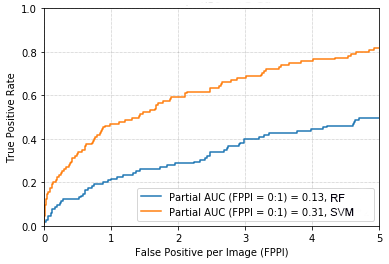
\includegraphics[width=8.5cm]{rf_svm_roc_lbp.png}}
%  \vspace{2.0cm}
\end{minipage}
  \label{fig:res_lbp}
\end{figure}
    
\begin{figure}[htb]
\caption{FROC Curve using all features except LBP comparing the RF and SVM classifiers.}
\begin{minipage}[b]{1.0\linewidth}
  \centering
  \centerline{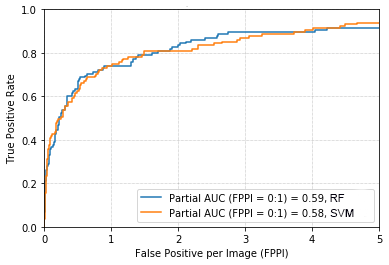
\includegraphics[width=8.5cm]{rf_svm_roc.png}}
%  \vspace{2.0cm}
\end{minipage}
 \label{fig:res_no_lbp}
\end{figure}

\section{Discussion}

As mentioned in the previous section, out of 115 masses in the database, the employed prepossessing and segmentation method correctly identified 110 regions. Therefore, the FROC curve never reaches its full potential as one, instead reaching a maximum of 0.956. When performing segmentation, detection of all positive regions and the increase of false positive regions was found to be a major trade-off. A slightly different approach on the prepossessing stage is anticipated to improve the segmentation in future works. Moreover, post-processing of segmented regions can be applied later.


The performance of both SVM and RF classifiers was carefully scrutinized for features obtained with and without LBP. As can be seen in \ref{fig:res_no_lbp}, both classifiers perform similarly (Partial AUC $\approx 0.59$ for RF and $\approx 0.58$ for SVM) on all features with the exception of LBP. But for the set of features including LBP, SVM proved to have a significantly higher performance in comparison to RF even though the Partial AUC was much lower than the previous case (see Figure \ref{fig:res_lbp}) for reasons stated above.


Additionally, the limited number of the positive mass images and diagnostic reports posed a great challenge for the classifier, as it created an imbalanced class problem. Consequently, it was difficult to raise the AUC of both classifiers, while overcoming the class imbalance. Although basic classifiers are generally encouraged for such problems, a more complex approach might give improved results. Ideally, obtaining a larger image database with more positive samples is the best way to improve the classification model. 


\section{Conclusion}
\label{sec:print}
In this project, a system was proposed for automated mass detection in mammogram images, with the potential to provide crucial assistance to radiologists. In our method, we realized preprocessing of full images, segmentation of the ROIs, and successive classification based on predefined features. The source code of our method implementation was can be found on \texttt{GitHub} \cite{IMMAS2018}. In the future, improvement of this module could be made using a larger dataset with more positive cases, as well as an additional, more precise segmentation technique, perhaps using the VFC Snake model.
Moreover, in real radiology practice, physicians do not analyze images as unrelated entities, but a full diagnostic comprises the comparison between different mammogram views and previous studies. Implementing this kind of reasoning in CAD systems could represent a major improvement in their performance. The development of CAD systems that can facilitate and assist in real time mammogram analysis is challenging but has the potential to make a vast impact on radiology practice.\par








% Below is an example of how to insert images. Delete the ``\vspace'' line,
% uncomment the preceding line ``\centerline...'' and replace ``imageX.ps''
% with a suitable PostScript file name.
% -------------------------------------------------------------------------


% To start a new column (but not a new page) and help balance the last-page
% column length use \vfill\pagebreak.
% -------------------------------------------------------------------------
%\vfill
%\pagebreak

%\subsubsection{REFERENCES}
\label{sec:ref}

% References should be produced using the bibtex program from suitable
% BiBTeX files (here: strings, refs, manuals). The IEEEbib.bst bibliography
% style file from IEEE produces unsorted bibliography list.
% -------------------------------------------------------------------------

\begin{figure*}
    \centering
    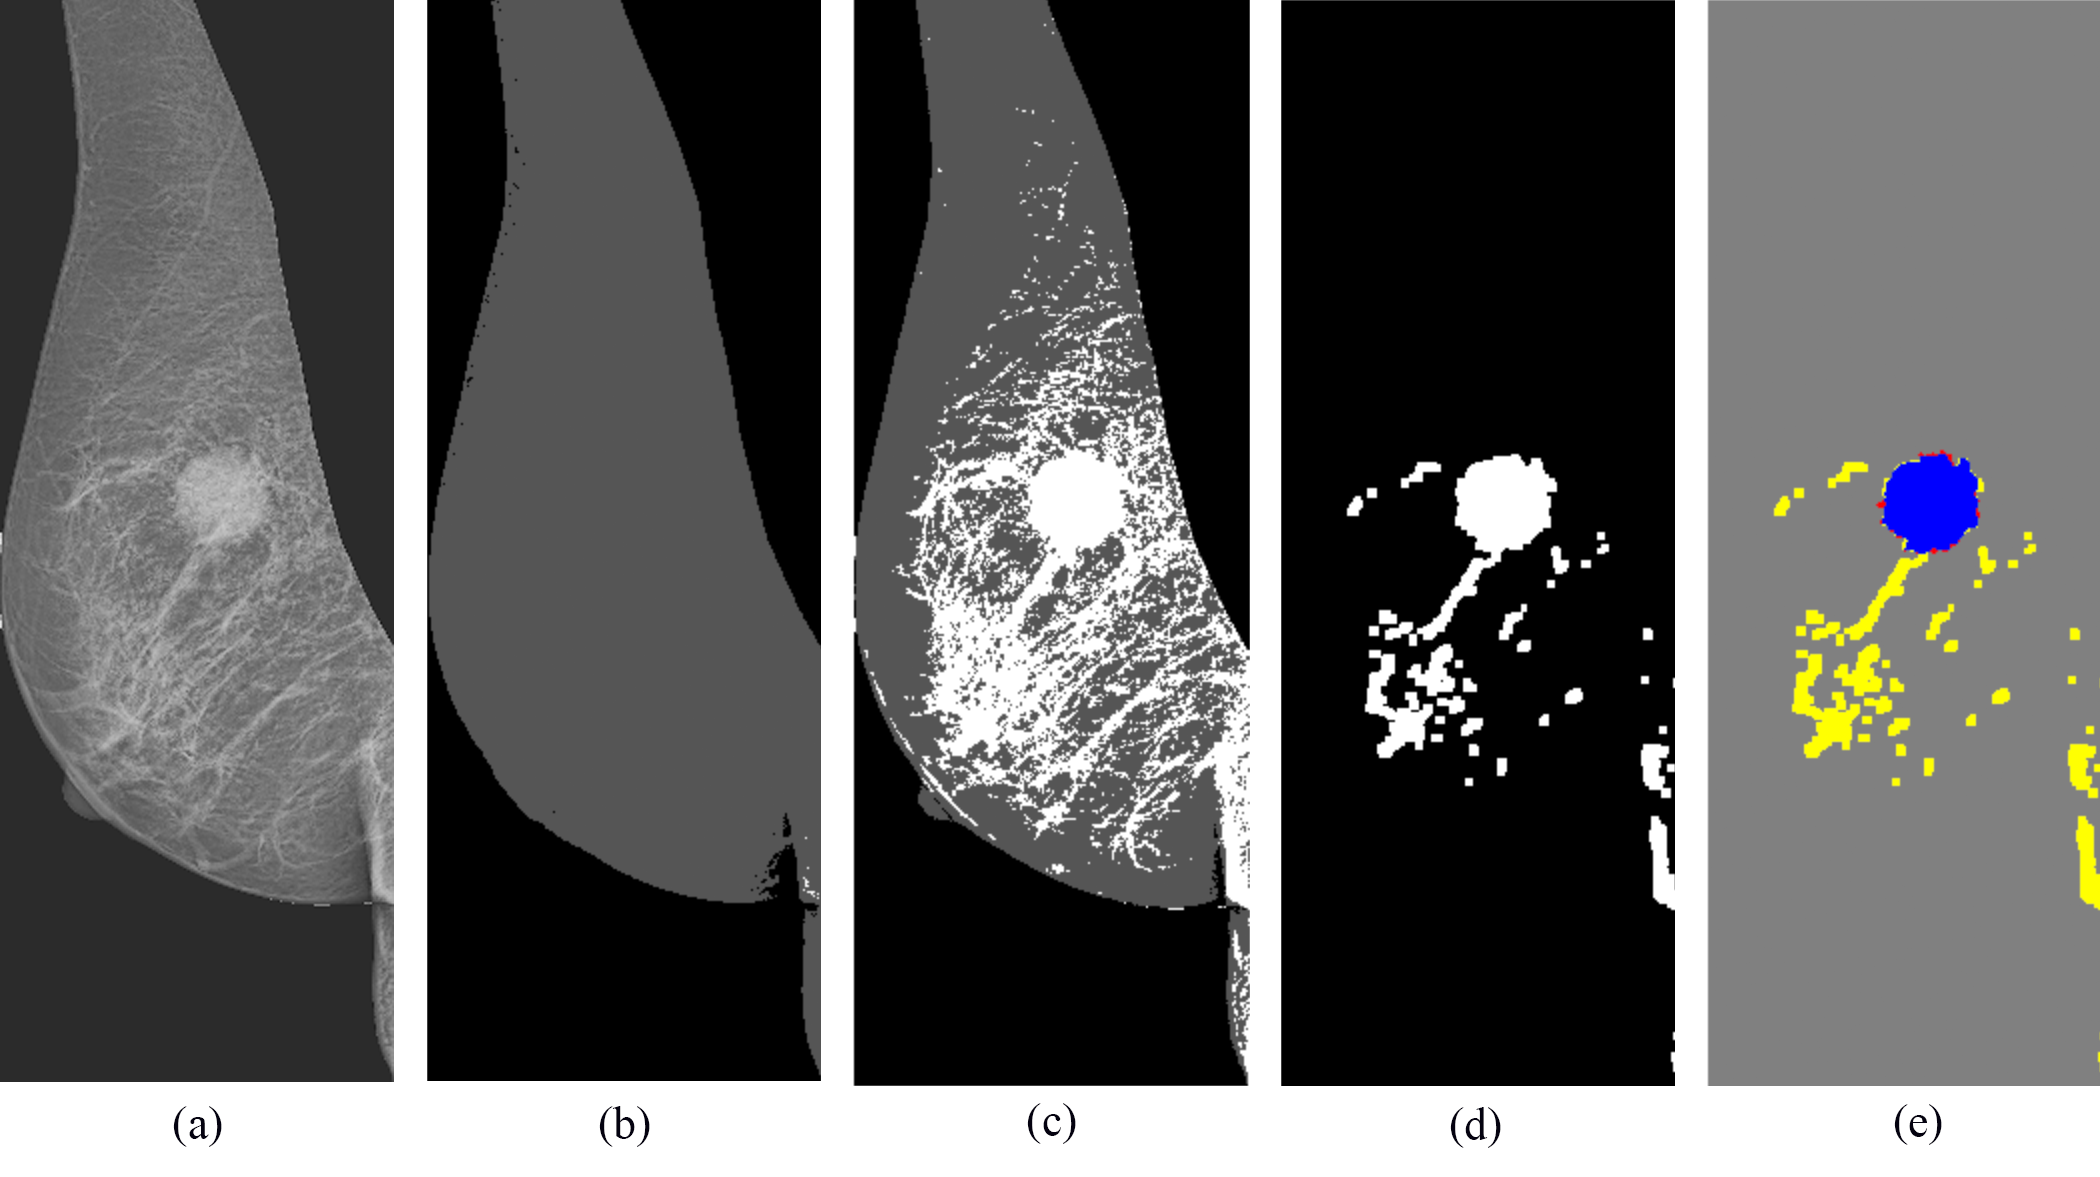
\includegraphics[width=6in]{segmentation_effect.png}
    \caption*{\textbf{Intermediate Result (IR) 1. }Effect of optimized preprocessing and segmentation on the regions. (a) original preprocessed image, (b) multithresholding without preprocessing, (c) multithresholding with preprocessing, (d) full segmentation method, including multithresholding and then cleaning on a preprocessed image, and (e) overlap of the segmented image from (d) with the groundtruth image. Blue represents true positive, red false negative, yellow false positive, and gray true negative. The overlapping blue region gives the maximum Jaccard index for this image.}
    \label{fig:lots_segmentation}
\end{figure*}

\bibliographystyle{IEEEbib}
\bibliography{MyCollection}





\begin{figure}
    \centering
    \caption*{\textbf{IR 2. }Histogram of Maximum Jaccard Index per image for segmented mass regions. Frequency vs. Jaccard Index}
    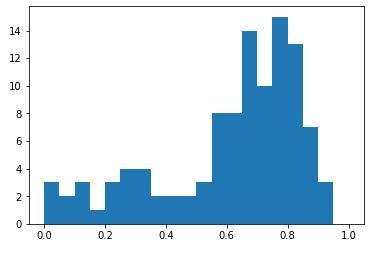
\includegraphics[width=8.5cm]{Jaccard_histogram.JPG}
    \label{fig:histogramjaccard}
\end{figure}


\begin{table}[]
\centering
\caption*{\textbf{IR 3. }Maximum area under the ROC curve obtained while optimizing hyperparameters for the SVM classifier}
\label{auc-results}
\begin{tabular}{lll}
\hline
\textbf{Kernel} & \textbf{No LBP} & \textbf{All Features} \\ \hline
RBF             & 0.9436                & 0.8954          \\
Sigmoid         & 0.9442                & 0.8905          \\
Linear          & 0.9429                & 0.8666          \\
Polynomial      & 0.9422                & 0.8969         \\ \hline
\end{tabular}
\end{table}










\end{document}